\documentclass[%
 preprint,
 amsmath,
 amssymb,
 aps,
]{revtex4-2}

\usepackage{graphicx}% Include figure files
\usepackage{dcolumn}% Align table columns on decimal point
\usepackage{bm}% bold math
\usepackage{lipsum}
\usepackage{physics}


\bibliographystyle{apsrev4-2}

\begin{document}
\title{New Progress on the Band Structure of $^{163}$Lu \\Paper Proposal}
\maketitle
\section{draft structure}
\begin{enumerate}
    \item Lucrul esential pe care l-am scos in evidenta in noile rezultate este cel prin care benzile TSD1 si TSD4 sunt parteneri de paritate, pe langa conceptul de parteneri de signatura intre TSD1 si TSD2. Ne axam doar pe acest lucru?
    \item Parity partner bands este un concept pe care nu l-am mai intalnit in literatura de wobbling pana acum. Important este \textbf{cum argumentam ca acest considerent este \emph{superior} sau \emph{imbunatatit} fata de modelele deja existene pentru explicatia structurii celor 4 benzi TSD?}
    \item Hamiltonianul nostru are o forma destul de simpla, fara considerente de calcul microscopic, si totusi produce deviatii de la experiment foarte mici. Acest lucru este intarit si de rezultatele deja publicate in ultima lucrare (lurcu pe care l-au mentionat si recenzorii). Merita mentionat?
    \item De obicei se pleaca cu o introducere in care sunt prezentate \emph{some previous models/results}. La ce rezultate/lucrari/experimente sa facem referire in paper? 
    \item Merita sa refac o schita in genul celei de mai jos, care explica concret si vizual toate considerentele structurii celor patru benzi. Consider ca este util. Ok?
\end{enumerate}

\section{other suggestions}

\par Din moment ce doriti ca acesta sa fie un Rapid Communication catre PRC, in cele 4-5 pagini este nevoie sa punem cele mai importante informatii. Va reamintesc ca avem destul de multe figuri, si acestea sigur vor ocupa cam mult spatiu daca le lasam sub forma de grid. Cu alte cuvinte, as dori sa imi spuneti cate lucruri.

\begin{enumerate}
    \item Pentru fiecare sectiune, ma gandeam: \textbf{Introduction} - in care prezentam previous results sau un fel de motivare pentru care venim cu aceasta idee. \textbf{Theoretical framework} - plecam de la Hamitlonian, si descriem pasii pentru calculul energiilor de wobbling, considerand numerele fononice de wobbling $(n_{w_1},n_{w_2})$ pentru fiecare din cele patru benzi. \textbf{Results I - energies} - aici prezentam energiile pe care le-am obtinut din fit. \textbf{results II - classical trajectories} - aici vorbesc despre cum am ajuns sa obtinem traiectoriile "clasice". Aici o sa adaug figurile cu ellipsoidul dar si contour plots pentru $H_{min}$. 
    \item Ce major conclusions ar trebui sa pun in evidenta in acest paper?
    \item Lucrari/referinte inspre care sa ma intrept pentru partea teoretica de \textit{parity partners}?
\end{enumerate}

\section{Workflow}

Workflow-ul modelului.

\begin{figure*}[h]
    \centering
    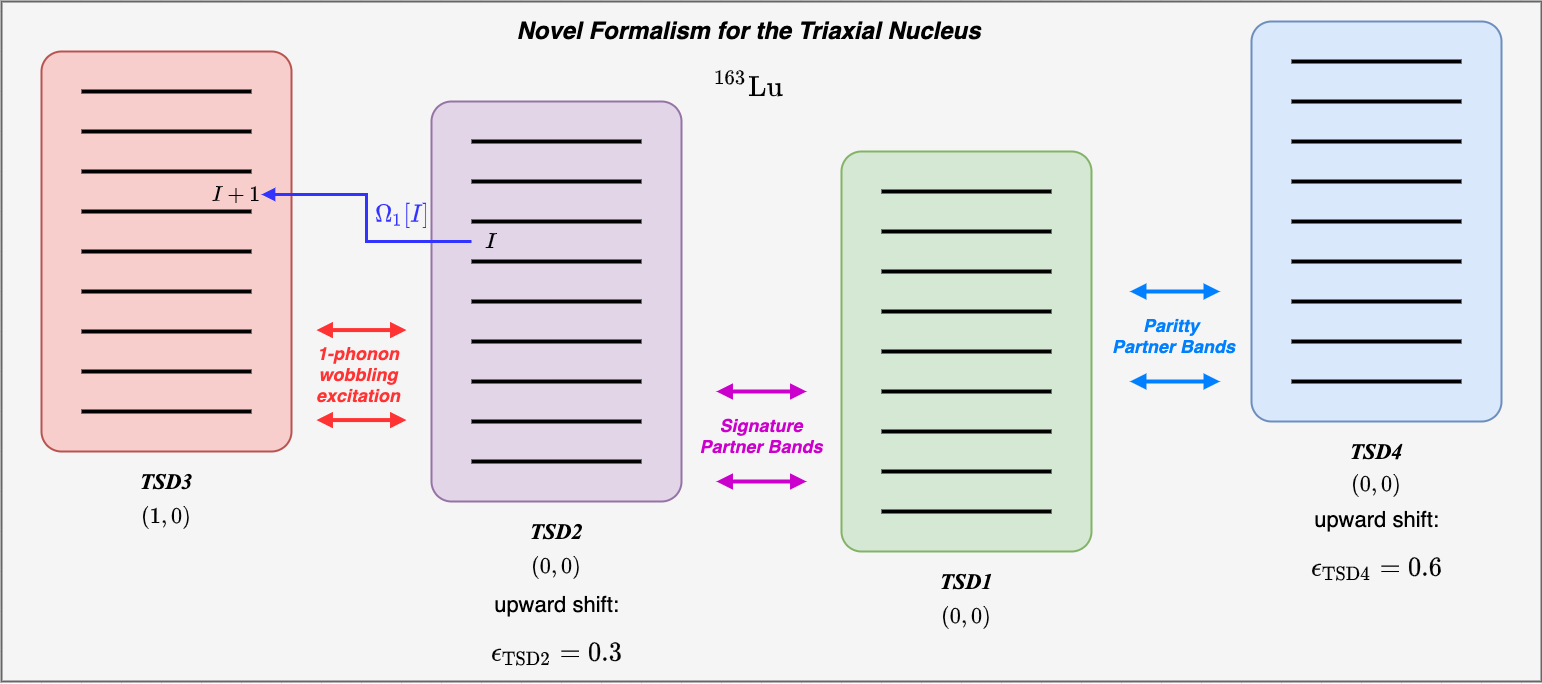
\includegraphics[width=0.95\textwidth]{images/diagrams/double_shift_fit_workflow.png}
    \caption{New approach}
    \label{fig:band-structure}
\end{figure*}

\end{document}